%---------------------------------------------------------------------------
\documentclass[
	a4paper,				% paper format
	10pt,					% fontsize 
	oneside,				% double-sided
	parskip=half,		% set paragraph skip to half of a line
]{style}						% style class
%---------------------------------------------------------------------------

% === doc details ===

\def\mytitle{Solar System Simulation}
\def\mytitlepicture{imgs/example_small.jpg} % title imagecd
\def\titlepicturelength{1\textwidth} % width of the image
\def\untertitle{Simulation of our solar system}
\def\type{Applications of Matlab/Octave}
\def\myname{Eric Lochmatter, Lukas Studer}
\def\myfield{Micro- and Medicaltechnology}
\def\mydate{06. 01. 2016}
\def\myabstract{{\em MatLab} and {\em Octave} are very versatile programs. To explore the possibilities, we created a simulation of our solar system using {\em MatLab}. bla bla bla realism, bla bla bla to scale and some shit about not elipsies but circles}


% ------------------------------------------------------------------------

\begin{document}

\maketitle %title
\frontmatter
\tableofcontents\thispagestyle{toc}
\mainmatter


% === main content ===
\chapter{Introduction}
This project aims at creating a simple modle of our solar system using {\em MatLab.} While putting emphasis on the visuals, we kept the mathematical aspect simple.

Trajectories are not calculated and the orbits are perfect circles, due to the simple fact that the difference would be hardly noticeable. The sizes and distances are mostly to scale. We use a logarithmic scale for the sizes and a linear, though a very small scale, for the distances. 
\pagebreak
\input{inputfiles/Realism.tex}
\chapter{UI Elements}

The modle provides two UI elements for the user, besides the common controls from {\em MatLab} itself. A display for the number of frames rendered pre second and a slider to control the speed at which the modle runs.

\section{FPS Display}
While programing the modle we soon realized that the certain changes had a massive impact on the number of frames {\em MatLab} could render per second. The number of frames per second, also known as {\em FPS} directally dictates how smooth the modle runs. Through time analysis of the modle we found out that the resolution of the planets, sun, and moon had the most noticable impact on the {\em FPS.} We then added the display to find the optimal resolution at which the graphics of the planets didn't suffer to much but still allowed for a smooth animation. We settled for a resolution of 50. This generates spheres composed of 50 equally wide rings with 50 equally big surfaces. This keeps the {\em FPS} around 20 which is only slightly lower than the number images the human eye can capture per secend. This makes the animation appear smooth. Following images shows how the sphreres react to different resolutions:

\begin{center}
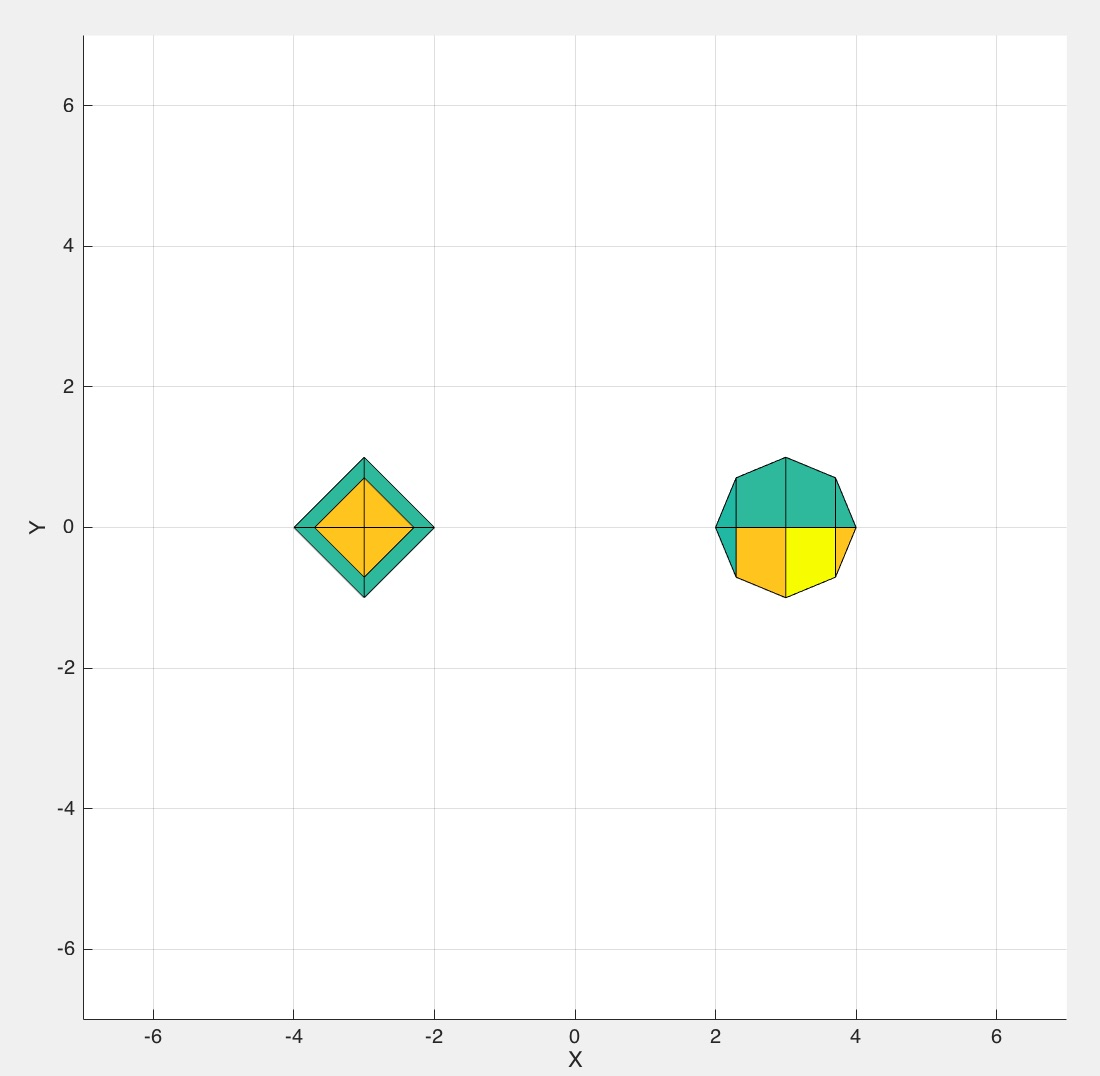
\includegraphics[width=0.45\textwidth]{imgs/ui_elements/spheres_res4.jpg}
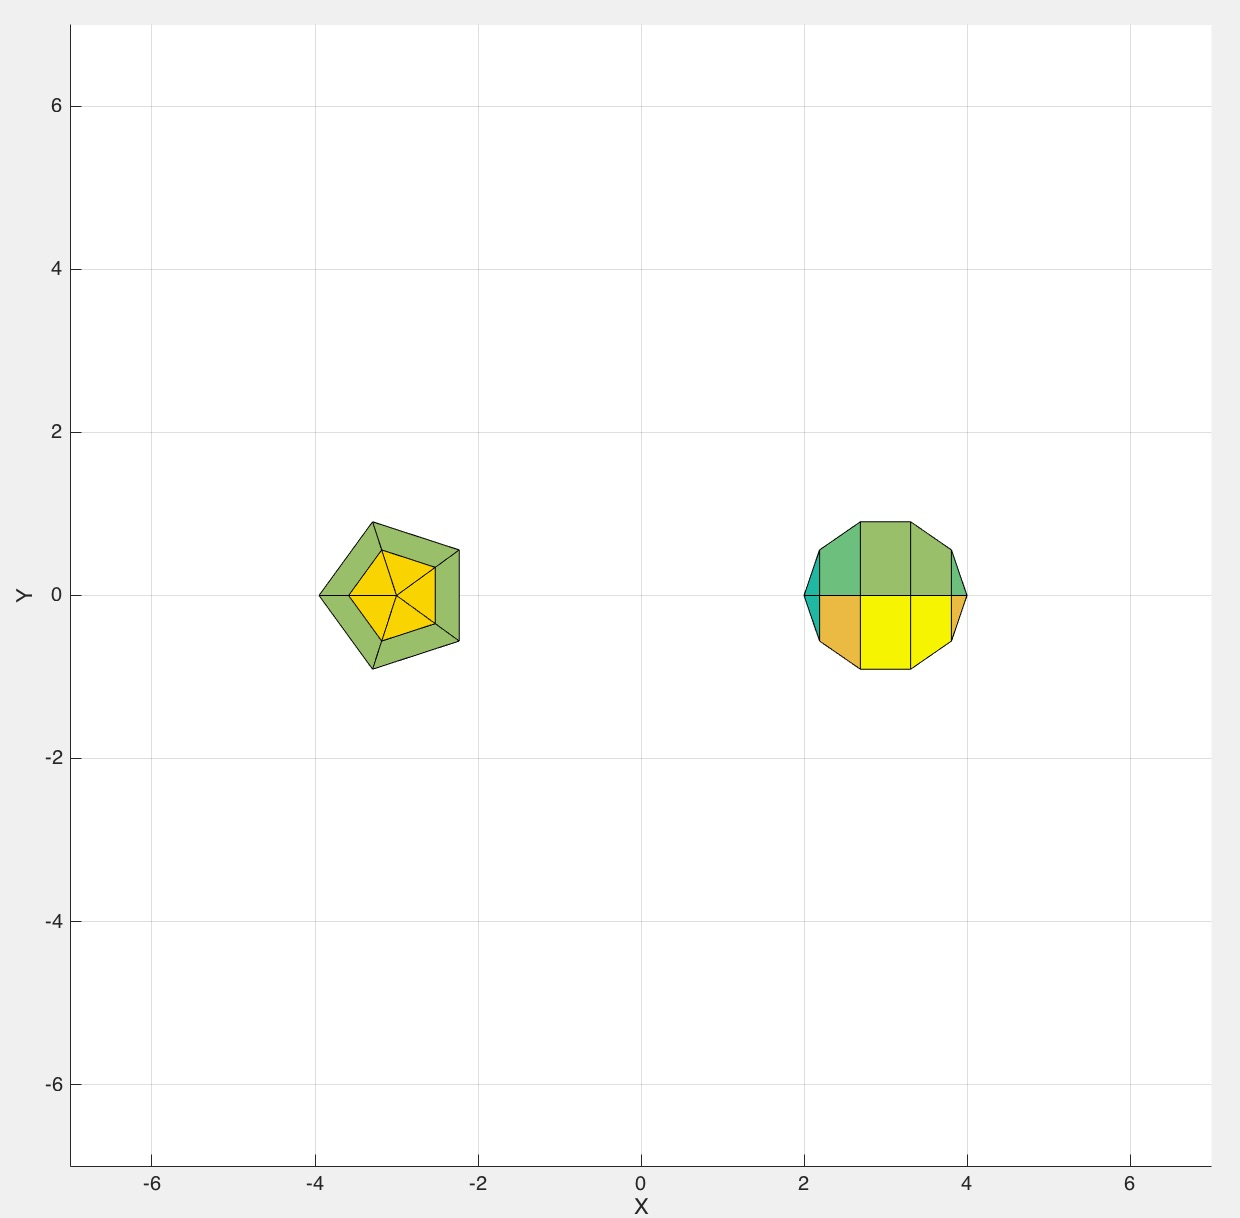
\includegraphics[width=0.45\textwidth]{imgs/ui_elements/spheres_res5.jpg}\\
\textit{Left: a sphere with resolution 4 (top and side view); Right: a sphere with resolution 5 (top and side view)}
\end{center}

\textcolor{red}{CALCULATION OF FPS}

\section{Speed Slider}
Because Uranus and Neptune are so far away from the sun, it takes them quite a while to complete an entire turn around the sun. That is why we added a slider on the bottom left which allows users to speed up the animation. Additionally the slider can also stop the animation by setting the speed to zero which allows for closer inspection of the planets. The slider basically controls the angle of rotation per tick. Faster speed results in a grater angle. Setting the speed to higher values leads to visual effects like planets appearing to jump rather than smoothly moving and planets smoothfully to be turning backwards. Alternatives like controling a delay for rendering the next frame have been tested, but didn't work out due to the {\em FPS} plummeting or the animation quickly reaching a maximum speed and therefore not having the desired effect.

\chapter{Rotation}

\section{The Problem with Rotation Angles}


\end{document}